\documentclass[../main.tex]{subfiles}
\begin{document}

This chapter presents and analyses a formal theoretical framework for truth
discovery. First, the approach taken is discussed and justified.

\section{Approach}
\label{sec:theory_approach}

In the previous chapters, we have motivated the need for a general theoretical
framework for truth discovery. To work towards actually constructing one, it is
necessary to set out exactly what such a framework will consist of, and what
features and properties are required for it to be useful.

The main goal of developing the framework is to set out rigorous definitions
for what truth discovery is, which allows the current situation to be modelled
whilst also permitting a more general view. The key definitions will therefore
be
\begin{itemize}
\item What is the `input' to truth discovery? The input has been described in
terms of sources, facts, objects and conflicting claims, but this needs to be
formulated mathematically.

\item What is the `output'? We have stated that the output is trust and belief
scores for sources and facts, according to the most common approach taken in
the literature. However our aim is to study truth discovery in full generality,
and not just the algorithms already in existence. Therefore a more general view
could be taken if desired, so long as it can still model existing algorithms.

\end{itemize}

With these definitions in place, a truth discovery algorithm is simply a
mapping from the space of inputs to outputs. This abstracts away the
\emph{process} of performing truth discovery so that `algorithm' is not the
correct term to use. We opt for \emph{truth discovery operator} to describe a
mapping from inputs to outputs.

There are several criteria against which to judge the usefulness of the
developed framework.
\begin{itemize}

\item \textbf{Ability to model existing approaches}: We aim to find a unified
framework that allow as many existing algorithms in the literature as possible
to be represented.

\item \textbf{Simplicity}: the key definitions should be easy to interpret, and
should relate to intuitive notions of truth discovery in a clear way.

\item \textbf{Flexibility}: we wish to prove properties of operators, compare
different operators, and develop axioms, so the framework should be easy and
flexible to work in.

\item \textbf{Generality}: the framework should be general and `unopinionated'
enough to be useful as foundations for future work, i.e. it should not rely on
specific ideas and approaches to performing truth discovery. It should also be
general in the sense of facilitating easy comparison between truth discovery
and related areas in the literature. This will allow ideas in these areas to be
applied to truth discovery, e.g. many axioms from social choice could be
translated to truth discovery.

\end{itemize}

Once the framework has been established, we aim to develop axioms for
operators. In line with axiomatic foundations for other problems, the axioms
should represent intuitively desirable properties that a `reasonable' operator
should satisfy. The power of the axiomatic approach is to then consider
multiple axioms together; the types of results attained include
\emph{impossibility results}, where it is proved that no operator\footnotemark
can satisfy a set of axioms, and \emph{representation theorems}, where a set of
sound and complete axioms are found for a particular operator. For example, in
\cite{altman_foundations} the authors show that two seemingly complementary and
desirable axioms cannot be satisfied simultaneously, which has implications
when deciding which ranking system to use in practise.

\footnotetext{
    We write `operator' as a blanket term to refer to social choice functions,
    ranking systems, annotation aggregators etc.
}

Requirements for `good' axioms include having simple interpretations and
representing desirable properties in some way or another.

To justify the decisions made in developing the framework, it is worth giving
an overview of the existing formalisms for truth discovery.

\subsection{Existing Formalisms}

The definitions of input in the popular truth discovery literature
\cite{li_survey, gupta_han_survey, pasternack, galland, zhang_qi_tang} are
generally compatible with each other: we have a set of sources and facts and
objects\footnotemark, and sources provide (or \emph{claim}) a set of facts for
objects. Some definitions are not in exactly this form, but can clearly be
restated in this form without changing the essence of the approach.

\footnotetext{
    Note that the terminology is not uniform across the literature; e.g. the
    survey in \cite{gupta_han_survey} refers to sources as `providers', and the
    facts in \cite{pasternack} are referred to as `claims' (i.e. the word
    `claim' is used as a noun, whereas we use it as a verb).
}

For example, in \cite{pasternack} there is no concept of objects, but instead
of \emph{mutual exclusion sets} of facts which cannot simultaneously be true.
However the mutual exclusion sets themselves can be seen as the objects linking
related facts together.

In \cite{galland}, there is no concept of objects, and sources may make
\emph{negative claims} where they state a fact is \emph{false}. However one may
view the `facts' (in the sense of \cite{galland}) as objects, and `true' and
`false' as the only two facts associated with each object.

There is more variety in the definitions of output. The treatment of sources is
generally the same: each source is assigned a \emph{trust score}, (usually a
number in $[0, 1]$), but differences appear for the treatment of facts. The two
main ideas are to assign each fact a \emph{belief score}, or to select a single
`true' fact for each object. Another view, taken in \cite{li_conflicts} for
example, is to produce a single value for each object to represent the true
fact, but where the true value may not have been claimed by any sources (for
example, a weighted average could be applied when facts are numeric values, and
could lead to this situation).

Selecting a single fact for each object can be seen as a special case of
assigning each fact a score; e.g. the true facts receive a score of 1 and all
others receive 0.

\subsection{Overview of Approach}
\label{sec:theory_approach_overview}

With this background in mind, we give an overview and justification of the
approach before the formal definitions are given in section
\ref{sec:theory_framework}.

For input, a graph-theoretic representation is chosen. Nodes will be sources,
facts and objects. Edges between nodes represent the obvious relations: an edge
from a source to a fact represents the source claiming that fact, and an edge
from a fact to an object indicates the object the fact relates to. Setting this
up in graph theory allows for simple interpretation, and allows concepts in
graph theory to be usefully applied to describe properties of the input (for
example, the notion of \emph{connected components} is key in axiom
\ref{axiom:indep}).

Using a well established tool such as graph theory is hoped to also provide
flexibility for future refinements to consider more complex problems: notions
such as weighted edges, annotated nodes etc. could be used to conveniently
describe additional properties of the input.

Finally, a graph representation is already used in the related area of ranking
systems \cite{altman_foundations, altman_personalised}. Using a similar set up
allows comparison between the two areas.

For output, consider the two main ideas discussed above: assigning each fact a
score and selecting a single true fact for each object. Since the latter is a
special case of the former, the former is more suitable for a general theory of
truth discovery.

Note that assigning a numeric score to each source and fact in particular
induces an \emph{ranking} of the sources and facts. We argue that the essence
of truth discovery lies more in this induced ranking that the particular
numerical scores, and will therefore define the output of truth discovery as a
pair of rankings (precisely, total preorders) on the set of sources and facts.

Indeed, when applying truth discovery methods to determine which sources to
trust and which facts to believe, one is interested in which sources/facts are
more believable than others, not in the particular numeric values produced by
an algorithm. Additionally, the numeric values produced often do not have any
semantic meaning \cite{pasternack}, which prevents inter-algorithm comparison.
The induced rankings can therefore act as a bridge between results from
different algorithms.

A similar view is also taken in social choice and the axiomatic theory of
ranking systems, where rankings instead of numeric scores are the main objects
of interest. Taking the same approach for here highlights the similarities
between truth discovery and these areas, and allows concepts in these areas to
be carried over into truth discovery.

Nevertheless, to model in their entirety the algorithms that produce numeric
scores, it will be possible to define such operators in the framework as more
general objects, but restrict our attention mainly to the ranking-output
operators.

\section{A Framework for Truth Discovery}
\label{sec:theory_framework}

In this section we define formally the graph-theoretic framework for truth
discovery, and set out the central problem of truth discovery via the
definition of a \emph{truth discovery operator}. We then develop axioms
(desirable properties) for such operators, and prove some basic properties
regarding them. Finally, we consider how to represent real-world truth
discovery algorithms in the developed framework, focussing specifically on
\emph{Sums} \cite{pasternack}.

First we state some standard definitions and notation.

\subsection{Standard Definitions and Notation}

\begin{definition}
A \emph{preorder} on a set $X$ is a binary relation $\preceq$ that is reflexive
and transitive:
\begin{enumerate}
\item $x \preceq x$ for all $x \in X$ (reflexivity)
\item If $x \preceq y$ and $y \preceq z$, then $x \preceq z$ for all $x, y, z
\in X$ (transitivity)
\end{enumerate}

A \emph{total preorder} is a preorder that is complete: for all $x, y \in X$,
$x \preceq y$ or $y \preceq x$. $\orderings(X)$ is the set of all total
preorders on $X$.

The \emph{strict} order induced by $\preceq$ is $\prec$ where $x \prec y$ if
and only if $x \preceq y$ but not $y \preceq x$. Note that $\prec$ is
irreflexive, transitive (and hence asymmetric), and is not complete.

The \emph{equality predicate} associated with $\preceq$ is $\simeq$, where $x
\simeq y$ if and only if $x \preceq y$ and $y \preceq x$. Note that $\simeq$ is
an equivalence relation on $X$.

\end{definition}

\begin{definition}
A \emph{permutation} of a set $X$ is a bijective mapping $X \rightarrow X$. We
use cyclic notation for permutations: $\pi=(a, b, c)$ is the mapping $\pi(a) =
b$, $\pi(b) = c$, $\pi(c) = a$, and $\pi(x) = x$ for $x \notin \{a, b, c\}$.
Juxtaposition of cycles denotes function composition.
\end{definition}

\begin{definition}

Two graphs $G=(V, E)$ and $G'=(V', E')$ are \emph{isomorphic} if there is a
bijective mapping $\phi: V \rightarrow V'$ such that $(u, v) \in E \iff
(\phi(u), \phi(v)) \in E'$.

\end{definition}

\begin{definition}
Let $G=(V, E)$ be an undirected graph, and define a relation $\sim$ on $V$ by
$u \sim v$ iff there is a path from $u$ to $v$ in $G$ (including the
zero-length path when $u = v$). It is easily checked that $\sim$ is an
equivalence relation. A \emph{connected component} of $G$ is an induced
subgraph of an equivalence class of $\sim$.
\end{definition}

\begin{notation}
For sets $X$ and $Y$, $Y^X$ denotes the set of all functions $X \rightarrow Y$.
\end{notation}

\subsection{Truth Discovery Definitions}

We consider fixed finite and mutually disjoint sets $\S$, $\F$ and $\O$, called
the \emph{sources}, \emph{facts} and \emph{objects} respectively. All
definitions and axioms will be stated with respect to these sets.

% Input network definition
\begin{definition}

A \emph{truth discovery network} is a directed graph $N = (V, E)$ where $V = \S
\cup \F \cup \O$, and $E \subseteq (\S \times \F) \cup (\F \times \O)$
satisfies the following properties:

\begin{enumerate}
\item Each $f \in \F$ has a unique successor node in $\O$, denoted $\obj(N, f)$
(i.e. each fact relates to a single object).

\item For $s \in \S$ and $o \in \O$, there is at most one directed path from
$s$ to $o$ (i.e. sources can only claim one fact per object).

\item $(\S \times \F) \cap E$ is non-empty (i.e. at least one claim is made).

\end{enumerate}
We will say that $s$ \emph{claims} a fact $f$ when $(s, f) \in E$. Let $\N$
denote the set of all truth discovery networks.
\end{definition}

\begin{remark}
Note that the definition above does not rule out a source $s$ making no claims,
a fact $f$ being claimed by no sources, or an object $o$ having no associated
facts or sources.

In the special case where each object has exactly two associated facts, the
objects can be seen as \emph{binary variables} taking one of two values, e.g.
true or false. The truth discovery network is then similar to a set of
judgements in \emph{judgement aggregation} \cite{handbook_ja} for an agenda
consisting only of propositional variables.
\end{remark}

\begin{notation}
For convenience, for a network $N=(V, E)$, define:
\begin{align*}
    \fact(N, s) &= \{f \in \F : (s, f) \in E\} \\
    \fact(N, o) &= \{f \in \F : (f, o) \in E\} \\
    \src(N, f) &= \{s \in \S : (s, f) \in E\} \\
    \src(N, o) &= \{s \in \S : \exists f \in \F : (s, f), (f, o) \in E\} \\
\end{align*}
\end{notation}

% Algorithm definition
\begin{definition}
\label{def:truth_discovery_operator}

A \emph{truth discovery operator} $T$ is a mapping $T: \N \rightarrow
\orderings(\S) \times \orderings(\F)$, i.e. $T$ assigns to each truth discovery
network $N$ a pair of total preorders $T(N) = (\sle_N^T, \fle_N^T)$ on the sets
$\S$ and $\F$ respectively.

$s_1 \sle_N^T s_2$ means $s_2$ is ranked as \emph{more trustworthy} than $s_1$
in the network $N$ according to $T$; $f_1 \fle_N^T f_2$ means $f_2$ is ranked
as \emph{more believable} than $f_1$.

\end{definition}

In practise, real-world truth discovery algorithms do not usually output a
ranking of sources and facts directly, but instead assign each source a numeric
\emph{trust score}, and each fact a \emph{belief score}. This is captured in
the following definition.

\begin{definition}
\label{def:numerical}

A \emph{numerical truth discovery operator} $T$ is a mapping $T: \N \rightarrow
\R^\S \times \R^\F$, i.e. $T$ assigns to each truth discovery network $N$
functions $t_N: \S \rightarrow \R$ (referred to as the \emph{source trust}
mapping) and $b_N: \F \rightarrow \R$ (referred to as the \emph{fact belief}
mapping).

\end{definition}

\begin{remark}
    Any numerical truth discovery operator $T$ naturally induces a
    truth discovery operator $T'$, where for any truth discovery network $N$
    we define
    \begin{align*}
    s_1 \sle_N^{T'} s_2 & \iff t_N(s_1) \le t_N(s_2) \\
    f_1 \fle_N^{T'} f_2 & \iff b_N(f_1) \le b_N(f_2)
    \end{align*}
    for $s_1, s_2 \in \S$ and $f_1, f_2 \in \F$.
\end{remark}

In this work we deal primarily with truth discovery operators as defined in
definition \ref{def:truth_discovery_operator}, instead of working directly with
numeric trust and belief scores as in definition \ref{def:numerical}. This is
due to the reasons dicussed in section \ref{sec:theory_approach_overview}; namely
that, from a theoretical point of view, we are interested in the qualitative
ranking of sources and facts rather than quantitative values.

One disadvantage to this approach is that whilst we can tell whether or not
$s_1$ is more trustworthy than $s_2$, we cannot tell by \emph{how much}. For
example, consider two numerical operators $T$ and $T'$ and $\S=\{s_1, s_2\}$
such that $t_N(s_1)=0.5, t_N(s_2)=0.51$, and $t_N'(s_1)=0.01, t_N'(s_2)=0.99$.
Both operators induce the same ranking on $\S$, yet $T$ considers the two
sources to have similar trust values while $T'$ considers $s_2$ to be much more
trustworthy than $s_1$.

\subsection{Axioms}
\label{sec:axioms}

The fact-believability component of truth discovery can be seen as a special
case of voting in the theory of social choice \cite{handbook_voting}, where
agents are sources and alternatives are facts. Each source then ranks the facts
it claims above all other facts, and ranks its claimed facts
equally\footnotemark. Several axioms for voting rules from this theory can be
adapted to truth discovery, and we do so presently.


\footnotetext{
    Note that the formulation of social choice must allow for agents to have
    \emph{weak} preferences for alternatives, where ties are allowed.
}

\subsubsection*{Symmetry and Dictatorship}

\begin{definition}
Two truth discovery networks $N$ and $N'$ are \emph{equivalent} if there is a
graph isomorphism $\pi$ between them that preserves sources, facts and objects:
\begin{enumerate}
\item $\pi(s) \in \S$ for all $s \in \S$
\item $\pi(f) \in \F$ for all $f \in \F$
\item $\pi(o) \in \O$ for all $o \in O$
\end{enumerate}

In such case we write $\pi(N)$ for $N'$.
\end{definition}

Figure \ref{img:equivalent_networks} shows an example of two equivalent
networks.

The first axiom states that the ordering of sources and facts should not depend
on the `names' of the sources, facts and objects in the input.

\begin{definition}
Let $T$ be a truth discovery operator. $T$ satisfies \emph{symmetry} if for
any equivalent truth discovery networks $N$ and $N' = \pi(N)$, we have
$$ s_1 \sle_N^T s_2 \iff \pi(s_1) \sle_{N'}^T \pi(s_2) $$
and
$$ f_1 \fle_N^T f_2 \iff \pi(f_1) \fle_{N'}^T \pi(f_2) $$

$T$ satisfies \emph{source-symmetry} if both the above statements hold in cases
where $\pi$ only permutes sources, i.e. $\pi(f)=f$ and $\pi(o)=o$ for all $f
\in \F$ and $o \in \O$. \emph{Fact-symmetry} and \emph{object-symmetry} are
defined similarly.
\end{definition}

\begin{axiom}[Symmetry]
\label{axiom:symm}
An operator $T$ should satisfy symmetry.
\end{axiom}

Source-symmetry is analogous to \emph{anonymity} in classical social choice,
where all voters are treated identically, and fact and object symmetry are
analogous to \emph{neutrality}, where the alternatives being
voted on are treated identically \cite{handbook_voting}.

Note that source-symmetry does not mean that sources are treated \emph{equally}
per se, since some sources are presumed to be more trustworthy than others
(this is more or less the central premise of truth discovery). Instead it means
that sources are judged solely by the facts that they claim, not their
identities.

\begin{figure}
    \centering
    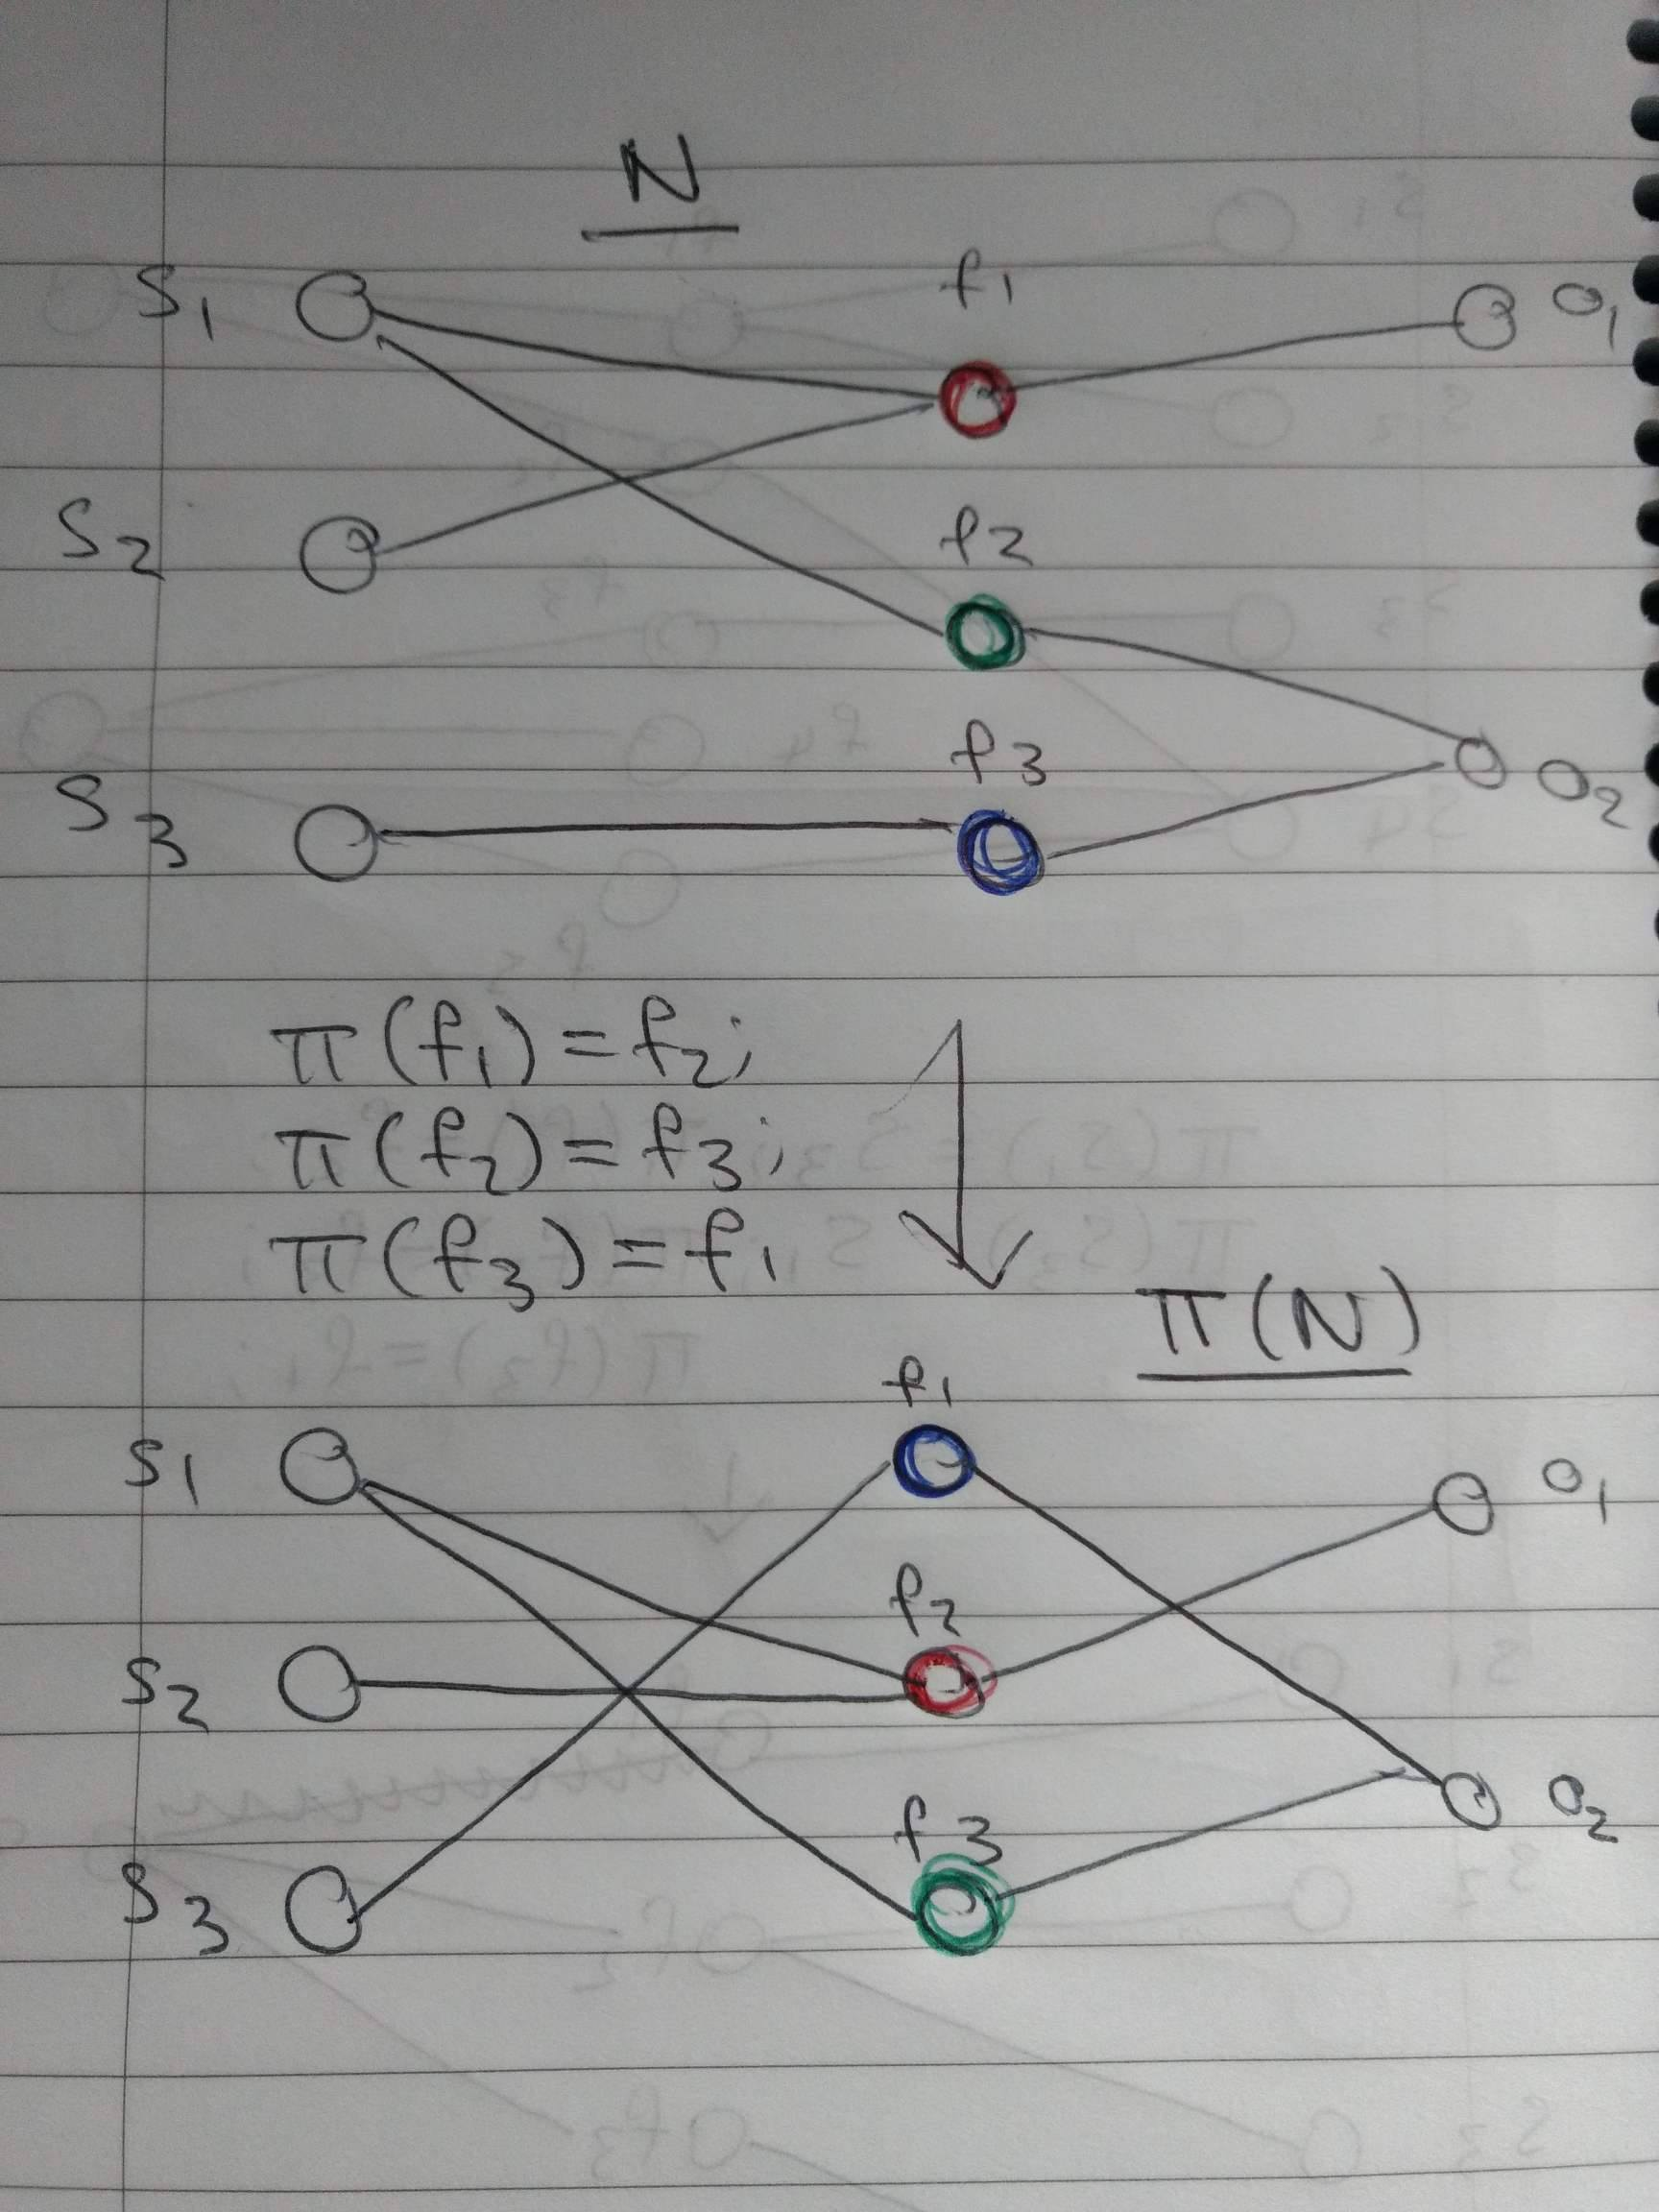
\includegraphics[width=\linewidth]{symmetry_example}
    \caption{
        Example of two equivalent truth discovery networks. Here the
        isomorphism between the left and right networks is $\pi = (S, T, U)(A,
        B)$. The colours show that the structure of the right network is the
        same as the left, just with different `names' for the nodes.
    }
    \label{img:equivalent_networks}
\end{figure}

\begin{proposition}
\label{prop:symm_iff_fact_source_object_symm}
$T$ satisfies symmetry if and only if it satisfies source, fact and object
symmetry.
\end{proposition}

\begin{proposition}
\label{prop:same_facts_ranked_equally}
If $T$ satisfies source-symmetry and $\fact(N, s_1) = \fact(N, s_2)$ in some
network $N$, then $s_1 \seq_N^T s_2$.

Similarly, if $T$ satisfies fact-symmetry and $\src(N, f_1) = \src(N, f_2)$,
$\obj(N, f_1) = \obj(N, f_2)$, then $f_1 \feq_N^T f_2$.

That is, any two sources making identical claims are ranked equally, and any
two facts for the same object with identical support from sources are ranked
equally.
\end{proposition}

All missing proofs are presented in appendix \ref{appendix:proofs}.

In some sense the opposite of source-symmetry, where the identities of the
sources are irrelevant and only the structure of the truth discovery network is
important, is a situation where \emph{only} the identities of the sources are
considered.

\begin{definition}

A source $s^* \in \S$ is \emph{authoritative} for a network $N=(V, E)$ with
respect to an operator $T$ if $s \sle_N^T s^*$ for all $s \in S$, and $(s^*,
f^*) \in E$ implies $f \fle_N^T f^*$ for all $f \in \F$.

In other words, $s^*$ is more (or equally) trusted than all other sources, and
its facts are more (or equally) believable than all others.

We also define a strict version: $s^*$ is \emph{strictly authoritative} if
additionally $s \slt_N^T s^*$ for all $s \ne s^*$, and $f \flt_N^T f^*$ for all
$f, f^* \in \F$ such that $(s^*, f^*) \in E$ and $(s^*, f) \notin E$.

An operator $T$ is a \emph{dictatorship} if there is a source $s^* \in S$ (the
dictator) that is authoritative for all networks, and $T$ is a \emph{strict
dictatorship} if there is a source $s^* \in S$ that is strictly authoritative
for all networks.

\end{definition}

\begin{axiom}[Non-dictatorship]
\label{axiom:non_dict}
An operator $T$ should not be a dictatorship.
\end{axiom}

As noted above, source-symmetry and dictatorship are conceptually at odds with
one another. This is expressed formally in the following proposition, which
essentially shows that only trivial operators can satisfy both properties.

\begin{proposition}
\label{prop:symm_and_dict}

If an operator $T$ is both source-symmetric and a dictatorship, then for any
network $N$:
\begin{enumerate}
\item All sources are ranked equally
\item If $f_1$ is claimed by at least one source in $N$, then $f_2 \fle_N^T
f_1$ for all facts $f_2$.
\end{enumerate}

In particular, there is no operator that is both source-symmetric and a strict
dictatorship.
\end{proposition}

\begin{example}
A trivial operator that satisfies symmetry and dictatorship is one that always
ranks all sources and facts equally: $T_{triv}(N) = (\S^2, \F^2)$.

If we restrict $\N$ to those networks where all facts are claimed by
at least one source, then proposition \ref{prop:symm_and_dict} shows that $T$
satisfies source-symmetry and dictatorship if and only if $T=T_{triv}$.

Without this restriction, facts not claimed by any source may be ranked
strictly below other facts. Indeed, consider $T$ defined as follows. For any
network $N$ write $F_{+} = \{f \in \F : \src(N, f) \ne \emptyset \}$, and
define $T$ by $s_1 \seq_N^{T} s_2 \text{ for all } s_1, s_2 \in \S$, and
$$
    f_1 \fle_N^{T} f_2 \iff f_2 \in F_{+} \text{ or } f_1 \notin F_{+}
    \quad
    (f_1, f_2 \in \F)
$$

$T$ is trivially a dictatorship for \emph{any} $s^* \in \S$. It can be easily
checked that $\fle_N^T$ is a well-defined total preorder, and that $T$ is also
symmetric. However any fact in $\F \setminus F_+$ ranks strictly below any fact
in $F_+$.
\end{example}

Dictatorship requires there to be a fixed source that is authoritative
in all networks. A weaker form of dictatorship, which is more compatible with
symmetry, is where the authoritative source may depend on $N$.

\begin{definition}
\label{def:gen_dict}
A truth discovery operator $T$ is a \emph{generalised dictatorship} if for
every network $N$ there exists a source $s_N \in \S$ that is authoritative for
$N$ with respect to $T$. A \emph{generalised strict dictatorship} is defined
similarly.
\end{definition}

Clearly a dictatorship is also a generalised dictatorship.

\begin{example}
\label{example:symm_and_gen_dict}
An operator that is both symmetric and a generalised dictatorship is the
numerical operator $T$ defined as follows. For any truth discovery network $N$,
let $Q_N = \{s \in \S \colon |\fact(N, s)| = \max_{x \in \S}{|\fact(N, x)|}\}$
be the set of sources making the maximal number of claims, and set
\[
    t_N(s) = \begin{cases}
        1 & \text{ if } s \in Q_N \\
        0 & \text{ otherwise}
    \end{cases}
\]
\[
    b_N(f) = \begin{cases}
        1 & \text{ if } \src(N, f) \cap Q_N \ne \emptyset \\
        0 & \text{ otherwise}
    \end{cases}
\]
Clearly any source in $Q_N$ is authoritative.

To show symmetry, let $N$ and $\pi(N)$ be equivalent networks. Let $s \in \S$.
First note that $f \in \fact(N, s)$ iff $\pi(f) \in \fact(\pi(N), \pi(s))$ by
definition of equivalent networks, and in particular the restriction of $\pi$
to $\fact(N, s)$ is a bijection into $\fact(\pi(N), \pi(s))$; hence $|\fact(N,
s)| = |\fact(\pi(N), \pi(s))|$. Also, since $\pi$ restricted to $\S$ is a
bijection into $\S$, we have
\begin{align*}
    \max_{x \in \S}{|\fact(N, x)|} & = \max_{x \in \S}{|\fact(\pi(N), \pi(x))|} \\
                                   & = \max_{x \in \S}{|\fact(\pi(N), x)|}
\end{align*}
\begin{align*}
    s \in Q_N & \iff |\fact(N, s)| = \max_{x \in S}{|\fact(N, x)|} \\
              & \iff |\fact(\pi(N), \pi(s))| = \max_{x \in S}{|\fact(\pi(N), x)|} \\
              & \iff \pi(s) \in Q_{\pi(N)}
\end{align*}
We see that $t_N(s) = t_{\pi(N)}(\pi(s))$ for any $s \in \S$.

Now let $f \in \F$. Note that $s \in \src(N, f)$ iff $\pi(s) \in \src(\pi(N),
\pi(f))$. Using this fact and $s \in Q_N \iff \pi(s) \in Q_{\pi(N)}$, it is
easy to see that $\src(N, f) \cap Q_N \ne \emptyset$ iff $\src(\pi(N), \pi(f))
\cap Q_{\pi(N)} \ne \emptyset$, i.e. $b_N(f) = b_{\pi(N)}(\pi(f))$.

Finally this means, for any $s_1, s_2 \in \S$ and $f_1, f_2 \in \F$:
\begin{align*}
    s_1 \sle_N^T s_2 & \iff t_N(s_1) \le t_N(s_2) \\
                     & \iff t_{\pi(N)}(\pi(s_1)) \le t_{\pi(N)}(\pi(s_2)) \\
                     & \iff \pi(s_1) \sle_{\pi(N)}^T \pi(s_2)
\end{align*}
and similarly $f_1 \fle_N^T f_2$ iff $\pi(f_1) \fle_{\pi(N)}^T f_2$. Hence $T$
is symmetric.
\end{example}

Note that to be a generalised dictatorship, an operator needs only to rank
facts claimed by the most trusted source(s) above all other facts. One may
argue that this is not necessarily an undesirable property, since the most
trusted source presumably claims believable facts, which \emph{should} rank
highly.

However, the operator in example \ref{example:symm_and_gen_dict} has the
additional (perhaps undesirable) property that the ranking is `binary': it is
two-level ranking where all non-authoritative sources rank equally to each
other and strictly below the authoritative ones. This behaviour is captured in
the following definition.

\begin{definition}
A truth discovery operator $T$ is a \emph{binary generalised dictatorship} if
for every network $N$ there is a set of sources $Q_N \subseteq \S$ such that,
with
\begin{align*}
    t_N(s) & = \begin{cases}
        1 & \text{ if } s \in Q_N \\
        0 & \text{ otherwise}
    \end{cases} \\
    b_N(f) & = \begin{cases}
        1 & \text{ if } \src(N, f) \cap Q_N \ne \emptyset \\
        0 & \text{ otherwise}
    \end{cases}
\end{align*}
it holds that
\[ s_1 \sle_N^T s_2 \iff t_N(s_1) \le t_N(s_2) \]
\[ f_1 \fle_N^T f_2 \iff b_N(f_1) \le b_N(f_2) \]

\end{definition}

\begin{remark}
If $T$ is a binary generalised dictatorship, it clear that for each network
$N$, each source in $Q_N$ is authoritative.

In such case the orderings $\sle_N^T$ and $\fle_N^T$ are fully determined by
the choice of $Q_N$. Therefore a binary generalised dictatorship can be
identified with a mapping $\N \rightarrow 2^\S$ that selects the authoritative
sources for each truth discovery network.
\end{remark}

\begin{axiom}[Non- binary generalised dictatorship]
\label{axiom:non_bin_gen_dict}
An operator $T$ should not be a binary generalised dictatorship.
\end{axiom}

\begin{proposition}
\label{prop:non_dict_and_non_bin_gen_dict_indep}
Non-dictatorship and non- binary generalised dictatorship are independent.
\end{proposition}

\subsubsection*{Unanimity}

The next axioms formalise the idea that if all sources are in agreement about
the status of a fact, then a truth discovery operator should respect this in
its verdict. Two obvious ways in which sources can be in agreement are when
\emph{all} sources believe a fact is true, and when \emph{no} sources believe a
fact is true.

\begin{axiom}[Unanimity]
\label{axiom:unanimity}
For any truth discovery network $N$, $\src(N, f) = \S$ implies $f' \fle_N^T f$
for all $f' \in \F$.
\end{axiom}

\begin{axiom}[Groundedness]
\label{axiom:groundedness}
For any truth discovery network $N$, $\src(N, f) = \emptyset$ implies $f
\fle_N^T f'$ for all $f' \in \F$.
\end{axiom}

That is, a fact cannot do better than to be claimed by all sources when $T$
satisfies unanimity, and cannot do worse than to be claimed by no sources when
$T$ is grounded.

Note that we do not require strict inequalities here, so as to not be too
restrictive. For unanimity in particular, requiring $f$ to rank strictly above
all other facts would require $T$ to choose a highest-ranking fact arbitrarily
in the case where there are multiple facts claimed by all sources.

Unanimity is similar to the \emph{weak Paretian} property \cite{handbook_intro}
in social choice, which states that whenever each individual prefers an
alternative $a$ over $b$, the social preference order prefers $a$ over $b$
also. It can also be compared to unanimity in judgement
aggregation \cite{handbook_ja}.

Axioms similar to groundedness have been proposed for collective annotation
(e.g. see \emph{groundedness} in \cite{kruger})

\todo{check social choice and JA incarnations of these principles}.

\begin{example}
The \emph{majority voting} operator, which ranks a fact by the number of
sources claiming it, satisfies unanimity and groundedness. Indeed, define
$T_{vote}$ by $s_1 \seq_N^{T_{vote}} s_2$ for all $s_1, s_2 \in \S$, and
    $$ f_1 \fle_N^{T_{vote}} f_2 \iff |\src(N, f_1)| \le |\src(N, f_2)| $$

If $\src(N, f) = \S$ then for all $f'$ we have $\src(N, f') \subseteq \S =
\src(N, f)$, so $f' \fle_N^T f$. Also, if $\src(N, f) = \emptyset$ then
$\src(N, f) \subseteq \src(N, f')$ for all $f'$, so $f \fle_N^T f'$. Hence
$T_{vote}$ is unanimous and grounded.
\end{example}

A consequence of groundedness is that any fact ranking strictly above all
others must have been claimed by at least one source (assuming $|\F|>1$).

\begin{proposition}
\label{prop:unam_ground_indep}
Unanimity and groundedness are independent.
\end{proposition}

\subsubsection*{Independence}

In social choice, the `Independence of Irrelevant Alternatives' (IIA) axiom
\cite{arrow} requires that the relative ranking of two alternatives $A$ and $B$
depends only on the individual rankings of $A$ and $B$, and not on any
`irrelevant' alternative $C$. That is, if the individual voter preferences are
changed such that the ranking of $A$ versus $B$ remains the same for each
voter, the ranking of $A$ and $B$ in the social ranking remains unchanged.

\begin{figure}
    \centering
    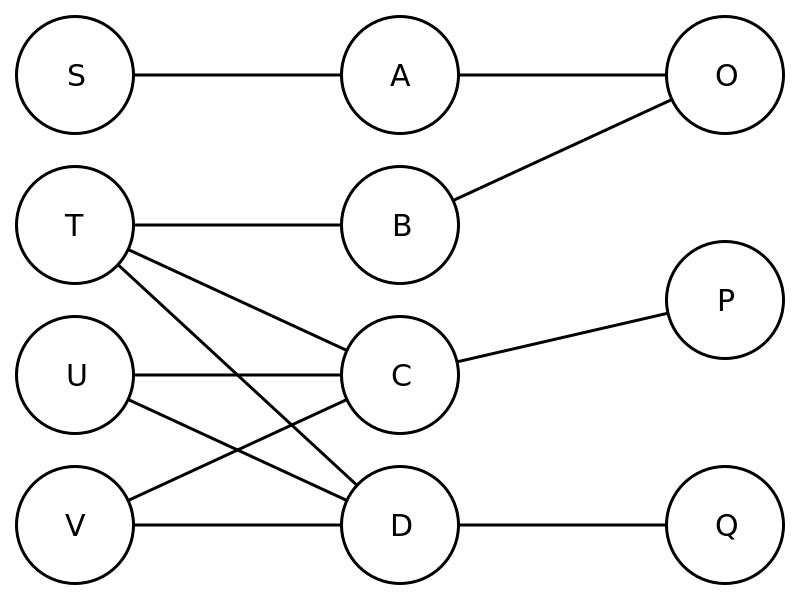
\includegraphics[width=25em]{independence_illustration_1}
    \caption{
        A network demonstrating a case where we do not wish for an IIA-type
        axiom to hold.
    }
    \label{img:independence_illustration_1}
\end{figure}

To consider whether a similar axiom should be adopted for truth discovery,
consider facts $A$ and $B$ in the network shown in figure
\ref{img:independence_illustration_1}. $A$ has support from source $S$ only,
who is not in agreement with any other sources, whilst $B$ has support from
$T$, who agrees with both $U$ and $V$ on facts $C$ and $D$. For this reason, it
may be reasonable to expect that $T$ is more trustworthy than $S$, and
therefore $B$ is more believable than $A$.

Directly translating IIA to this situation, we would require that the ranking
of $A$ and $B$ is unchanged if, say, we removed $T$'s claims for $C$ and $D$
(which are `irrelevant'), and instead had $S$ make these claims. However the
intuition above suggests that the ranking of $A$ and $B$ should actually be
\emph{reversed} in this case, despite the individual judgements on $A$ and $B$
remaining unchanged. For this reason, we argue that a more subtle notion of
independence is required.

\begin{figure}
    \centering
    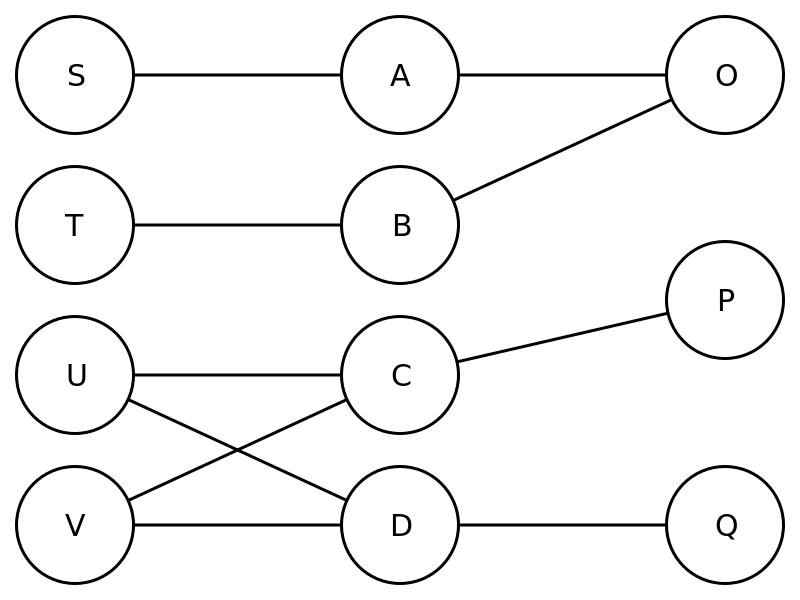
\includegraphics[width=25em]{independence_illustration_2}
    \caption{
        A network where some notion of independence may be applied
    }
    \label{img:independence_illustration_2}
\end{figure}

The issue in figure \ref{img:independence_illustration_1} is that $C$ and $D$
are not entirely irrelevant to $A$ and $B$, since they are connected indirectly
via sources that make claims for both objects $O$ and $P$ (namely, source $T$).
Consider removing these indirect links, as show in figure
\ref{img:independence_illustration_2}. In this case it can be argued that $C$
and $D$ truly are irrelevant to $A$ and $B$, and so changes to the network
outside of $S$, $T$, $A$, $B$ and $O$ should not affect the ranking of $A$ and
$B$.

This idea can be generalised by noting that two nodes are `relevant' to each
other (perhaps indirectly) if they lie in the same \emph{connected component}
of the network (where we consider the connected components of the undirected
version of the graph). A suitable independence axiom is therefore to require
that changes outside a connected component do not affect the ranking of sources
and facts within that component. A precise statement is given below.

\begin{axiom}[Independence Of Irrelevant Stuff]
\label{axiom:indep}
For any truth discovery networks $N_1$, $N_2$ with a common connected component
$G$, the restrictions of $\sle_{N_1}^T$ and $\sle_{N_2}^T$ to $G \cap \S$ are
equal, and the restrictions of $\fle_{N_1}^T$ and $\fle_{N_2}^T$ to $G \cap \F$
are equal.
\end{axiom}

Independence of irrelevant stuff requires that $s_1 \sle_{N_1}^T s_2$ if and
only if $s_1 \sle_{N_2}^T s_2$. A weaker version is to require only that the
ranking of $s_1$ and $s_2$ in $N_1$ is \emph{not reversed} in $N_2$, not
necessarily that the ranking if the same (for example, a strict inequality in
$N_1$ may become weak in $N_2$).

\begin{axiom}[Weak Independence Of Irrelevant Stuff]
\label{axiom:weak_indep}
For any truth discovery networks $N_1$, $N_2$ with a common connected component
$G$ and for any $s_1, s_2 \in G \cap S$ and $f_1, f_2 \in G \cap \F$:
\[
    s_1 \slt_{N_1}^T s_2 \implies s_1 \sle_{N_2}^T s_2
\]
\[
    f_1 \flt_{N_1}^T f_2 \implies f_1 \fle_{N_2}^T f_2
\]
\end{axiom}

Clearly axiom \ref{axiom:indep} implies axiom \ref{axiom:weak_indep}.

\subsubsection*{Coherence}

A guiding principle of many truth discovery approaches is that facts claimed by
trustworthy sources should receive high belief, and sources claiming high
belief facts should be seen as trustworthy -- the trust and belief rankings
should cohere with one another in this sense. The following axiom aims to
formalise this in a specific case where it is possible to compare facts for two
sources in a straightforward way (and similarly for facts).

\todo{Mention that this idea is from transitivity axioms in
\cite{altman_foundations}}

\begin{axiom}[Coherence]
Suppose $N$ is a truth discovery network and $s_1, s_2 \in \S$ are such that
there is a bijective mapping $\phi: \fact(N, s_1) \rightarrow \fact(N, s_2)$
with $f \fle_N^T \phi(f)$ for all $f \in \fact(N, s_1)$. Then $s_1 \sle_N^T
s_2$.

That is, if the facts claimed by two sources can be paired up such that the
fact claimed by $s_1$ always ranks beneath the fact claimed by $s_2$, then
$s_1$ ranks beneath $s_2$.

Similarly, if there are facts $f_1, f_2 \in \F$ and a bijection $\phi: \src(N,
f_1) \rightarrow \src(N, f_2)$ such that $s \sle_N^T \phi(s)$ for all $s \in
\src(N, f_1)$, then $f_1 \fle_N^T f_2$.

\end{axiom}

\todo{Come up with an example of a coherent operator}

\subsubsection*{Monotonicity}

The axioms considered so far have largely dealt with the output of a truth
discovery operator for one input network at a time, or for two networks which
are structurally similar. Another dimension to the axiomatic approach is to
consider how the output of an operator is effected by a \emph{change} in the
input to modify it in a particular way.

The following axiom considers what should happen if a network is changed by
adding additional support for a particular fact. Intuitively, this should be
seen as additional evidence that the fact is true, and an operator should rate
it no worse than it did before.

\todo{
    expand introductory note: compare to monotonicity in social choice, JA,
    annotation, trust recommendation
}

\begin{axiom}[Monotonicity]
Let $N = (V, E)$ be a truth discovery network, and $f \in \F$, $s \in \S$ such
that $(s, f) \notin E$. Write $o = \obj(N, f)$. Consider the network $N'=(V,
E')$ where $s$ claims $f$, i.e.
$$
    E' = \{(s, f)\} \cup E \setminus \{(s, f') : f' \ne f, (f', o) \in E\}
$$
Then $f' \fle_N^T f$ implies $f' \fle_{N'}^T f$ for all $f' \in \F$.

That is, if $f$ receives additional support from a new source $s$, its ranking
should not get worse.
\end{axiom}

\todo{Come up with an example of a monotonic operator }

\todo{Summary of all the axioms and any implications between them}

\todo{Analysis of majority voting: which axioms does it satisfy}

\subsection{Iterative Truth Discovery Operators}

Real-world algorithms for truth discovery generally compute numerical trust and
belief scores, as per definition \ref{def:numerical}. Additionally, most
operate in an \emph{iterative} manner, computing trust and belief scores
recursively from one another until the respective scores (hopefully) converge
to fixed values.

In this section we define the concept of iterative truth discovery operators to
represent and reason about such real-world algorithms.

\begin{definition}
\label{def:iterative_operator}

An \emph{iterative truth discovery operator} is a sequence $I=(T_n)_{n \in
\Nat}$ of numerical truth discovery operators, i.e. a sequence of mappings $T_n
: \N \rightarrow \R^\S \times \R^\F$.

For a network $N$ and $n \in \Nat$ we will write $T_n(N) = (t_N^n, b_N^n)$ to
refer directly to the source trust and claim belief mappings for the $n$-th
iteration (but note that this notation does not make explicit the dependence of
$t$ and $b$ on the sequence $I$).

$I$ is said to \emph{converge} to a numerical operator $T^*$ if $t_N^n
\rightarrow t_N^*$ and $b_N^n \rightarrow b_N^*$ pointwise as $n \rightarrow
\infty$ for each network $N$.

\end{definition}

\begin{remark}
Recall that a numerical operator $T^*$ naturally induces a (non-numerical)
operator by rankings sources according to $t_N^*$ and facts according to
$b_N^*$. We may therefore identify a convergent iterative operator $I$ with the
operator induced by its limit $T^*$, and write $\sle_N^I$ and $\fle_N^I$ for
the source and fact rankings. To be explicit:

$$ s_1 \sle_N^I s_2 \iff \lim_{n \rightarrow \infty}{t_N^n(s_1)} \le \lim_{n
\rightarrow \infty}{t_N^n(s_2)} $$

and similarly for facts.

Note that this mapping is not injective: there may be many iterative operators
with the same limit $T^*$; furthermore two distinct numerical operators $T^*$
and $T^{**}$ may induce the same non-numerical operator.
\end{remark}

Given a real-world algorithm in practise, one usually aims to determine whether
it converges by iterating until the distance (measured in some suitable way)
between trust (or belief) scores in consecutive iterations becomes smaller than
a fixed threshold. This is of course only a heuristic, since it is not possible
to determine whether a sequence converges by considering only finitely many
terms. Moreover even if the difference between subsequent trust/belief scores
were to become \emph{arbitrarily} small (i.e. smaller than \emph{any}
threshold), one still cannot guarantee convergence\footnotemark. This means
that it may not be trivial to define a real-world algorithm as a truth
discovery operator, since it may not be clear whether the trust and belief
scores converge in all cases. Nevertheless, in this work we will assume that
the iteration \emph{does} converge in all cases and consider which axioms of
section \ref{sec:axioms} are satisfied given this assumption.

\footnotetext{
    For an example of a sequence exhibiting such behaviour, consider the
    partial sums of the \emph{Harmonic series}
    $\sum_{j=1}^{\infty}\frac{1}{j}$, which is divergent. The difference
    between the $(n+1)$-th and $n$th terms is $\frac{1}{n+1}$ which converges
    to 0 as $n \rightarrow \infty$, yet the series does not converge.
}

To check whether a convergent operator satisfies the axioms, it will be
convenient to have sufficient conditions for some of the axioms that refer to
the numeric trust and belief scores directly.

For convenience we assume that trust and belief scores are in the range $[0,
1]$, as this is generally the case in practise.

\begin{lemma}
\label{lemma:iterative_axiom_suff_conds}
Let $I$ be a convergent iterative truth discovery operator with limit
$T^*$. Suppose that $t_N^n(s) \in [0, 1], b_N^n(f) \in [0, 1]$ for all $N, s,
f$ and $n$.

\begin{enumerate}
    \item $t_N^*(s) \in [0, 1]$ and $b_N^*(f) \in [0, 1]$

    \item If for any equivalent networks $N$ and $N'=\pi(N)$ it holds that
    \[
        t_N^n(s) = t_{\pi(N)}^n(\pi(s))
    \]
    and
    \[
        b_N^n(f) = b_{\pi(N)}^n(\pi(f))
    \]
    for all $N, n, s, f$, then $I$ satisfies symmetry (axiom \ref{axiom:symm}).

    \item If for any network $N$ and $f \in \F$,
    \[
        \src(N, f) = \S \implies b_N^n(f) = 1 \text{ for sufficiently large }
            n \in \Nat
    \]
    then $I$ satisfies unanimity (axiom \ref{axiom:unanimity}).

    \item If for any network $N$ and $f \in \F$,
    \[
        \src(N, f) = \emptyset \implies b_N^n(f) = 0
            \text{ for sufficiently large } n \in \Nat
    \]
    Then $I$ satisfies groundedness (axiom \ref{axiom:groundedness}).

    \item If for any networks $N_1$, $N_2$ with a common connected component
    $G$ it holds that $t_{N_1}^n(s) = t_{N_2}^n(s)$ and $b_{N_1}^n(f) =
    b_{N_2}^n(f)$ for $s \in G \cap \S$ and $f \in G \cap \F$, then $I$
    satisfies independence of irrelevant stuff (axiom \ref{axiom:indep}).

    \item If for any networks $N_1$, $N_2$ with a common connected component
    $G$ there are sequences of non-negative numbers $(\alpha_n)_{n \in \Nat}$,
    $(\beta_n)_{n \in \Nat}$ such that, for all $n \in \Nat$, $s \in G \cap \S$
    and $f \in G \cap \F$,
        \[ t_{N_2}^n(s) = \alpha_n \cdot t_{N_1}^n(s) \]
        \[ b_{N_2}^n(f) = \beta_n \cdot b_{N_1}^n(f) \]
    then $I$ satisfies weak independence of irrelevant stuff (axiom
    \ref{axiom:weak_indep}).

\end{enumerate}
\end{lemma}

\subsubsection*{Sums}

Sums \cite{pasternack} is an iterative algorithm for truth discovery based on
the Hubs and Authorities \cite{kleinberg} algorithm for the ranking of web
pages based on the hyperlink structure of the web. The trust score for a source
at a given iteration is computed as the sum of the current belief scores of its
claimed facts, and the belief score for a fact is given by the sum of its
sources trust scores.

The trust/belief scores are normalised at each iteration by dividing by the
maximum score; this prevents the scores growing without bound to ensure
convergence.

\begin{definition}[Sums]
Sums is the iterative truth discovery operator $I_{sums}$ defined for any
network $N$ as follows, where we write $t_n$ for $t_N^n$ for brevity:
\[
    t_1(s) = \frac{1}{2}, \quad b_1(f) = \frac{1}{2}
\]
and for $n > 1$:
\begin{align*}
    \hat{t}_n(s) & = \sum_{f \in \fact(N, s)}{b_{n - 1}(f)} \\
    \hat{b}_n(f) & = \sum_{s \in \src(N, f)}{\hat{t}_n(s)} \\
    t_n(s) & = \frac{\hat{t}_n(s)}{\max\limits_{x \in \S}{\hat{t}_n(x)}} \\
    b_n(f) & = \frac{\hat{b}_n(f)}{\max\limits_{y \in \F}{\hat{b}_n(y)}}
\end{align*}

Note that $\hat{t}$ and $\hat{b}$ are only used to define $t$ and $b$, and are
not part of the definition of Sums itself.

If a source $s$ makes no claims in $N$ (i.e. $\fact(N, s) = \emptyset$), we
follow the convention that an empty sum is 0 and set $\hat{t}_N^n(s)=0$
(similar for a fact without sources).
\end{definition}

\begin{remark}
The normalisation ensures that trust and belief scores always lie in $[0, 1]$.
Note that any source that makes at least one claim has strictly positive trust
score for all $n$, and any fact with at least one source has strictly positive
belief score. Since any network $N$ must contain at least one claim, this
ensures that the maximum in the denominator for $t_n$ and $b_n$ is non-zero.
\end{remark}

\begin{theorem}
\label{theorem:sums_axioms}
If Sums is convergent, it satisfies symmetry (axiom \ref{axiom:symm}),
non-dictatorship (axiom \ref{axiom:non_dict}), unanimity (axiom
\ref{axiom:unanimity}), groundedness (axiom \ref{axiom:groundedness}) and
weak independence of irrelevant stuff (axiom \ref{axiom:weak_indep}).
\end{theorem}

\begin{figure}
    \centering
    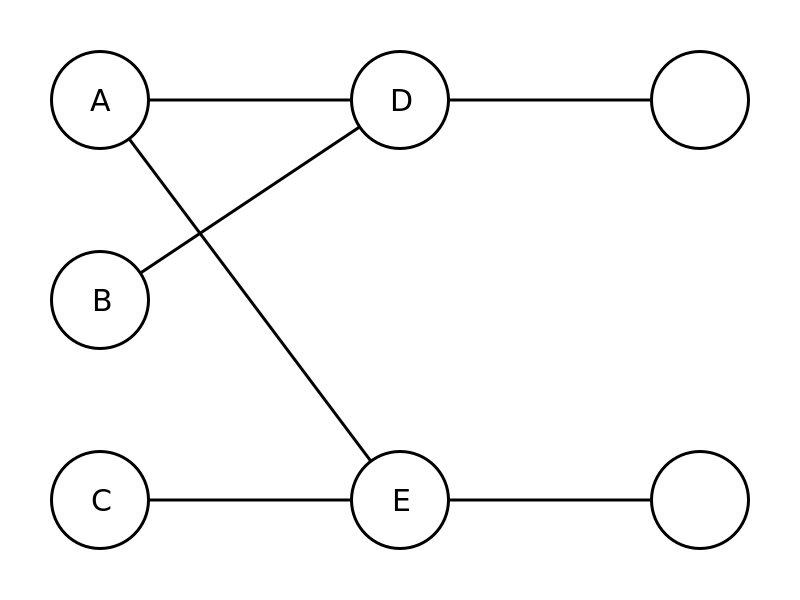
\includegraphics[width=25em]{sums_not_all_equal_trust}
    \caption{Network in which Sums does not rank all sources equally}
    \label{img:sums_not_all_equal_trust}
\end{figure}

The proof of theorem \ref{theorem:sums_axioms} uses lemma
\ref{lemma:iterative_axiom_suff_conds}, and can be found in appendix
\ref{appendix:proofs}. For non-dictatorship, it is sufficient by proposition
\ref{prop:symm_and_dict} and symmetry to find a single truth discovery network
in which Sums does not rank all sources equally. Figure
\ref{img:sums_not_all_equal_trust} shows such a network: in this network $A$
ranks strictly above $B$ and $C$, which are ranked equally.

\begin{theorem}
\label{theorem:sums_non_indep}
Sums does not satisfy Independence of Irrelevant Stuff (axiom
\ref{axiom:indep}).
\end{theorem}

\begin{figure}
    \centering
    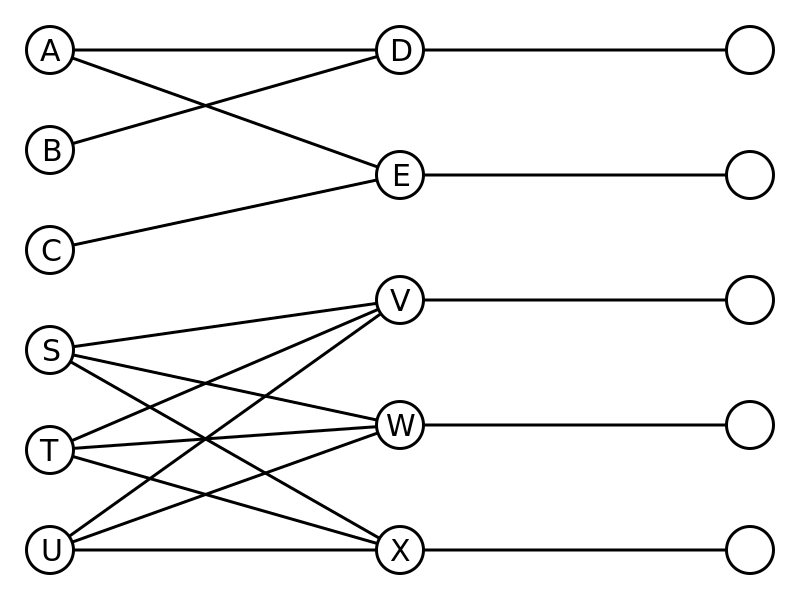
\includegraphics[width=25em]{sums_non_independence}
    \caption{
        Counter-example to independence for Sums: this network contains the one
        show in figure \ref{img:sums_not_all_equal_trust} as a connected
        component, but $A$ is ranked equal to $B$ here whereas it ranks
        strictly above $B$ in figure \ref{img:sums_not_all_equal_trust}.
    }
    \label{img:sums_non_indep}
\end{figure}

Figures \ref{img:sums_not_all_equal_trust} and \ref{img:sums_non_indep}
provide an example of Sums failing to satisfy independence. The details can be
found in the proof in appendix \ref{appendix:proofs}.

We conjecture that Sums is indeed convergent for any input network. Indeed, it
is easy to see that Sums closely related to Hubs and Authorities
\cite{kleinberg}, where trust scores correspond to hub scores, and belief
scores correspond to authority scores. There are only two differences: the
initial scores ($\frac{1}{2}$ in Sums and 1 in Hubs and Authorities), and the
method of normalisation (Sums ensures the maximum score is 1, whereas Hubs and
Authorities ensures the sum of the squares of the scores is 1). In
\cite{kleinberg} is is proved that Hubs and Authorities always converges using
techniques from linear algebra. The difference in normalisation only amounts to
using a different norm to measure convergence (namely $\|.\|_{\infty}$ in Sums
instead of $\|.\|_2$), so it is hoped that the proof can be modified to work
for Sums.

\section{Evaluation}

In this section, the framework and results of the previous section are
evaluated. In particular, the framework is evaluated with respect to the
criteria outlined in section \ref{sec:theory_approach}.

\subsection*{Ability to model existing approaches}

The main definitions are that of a truth discovery network and a truth
discovery operator. For the framework to be useful as tool for analysing truth
discovery, these definitions should be compatible with the existing ideas and
approaches to truth discovery, in the sense that it should be possible to
define existing algorithms within the framework.

For the input network definition, it is easily verified that the definition
given is capable of modelling the input required for many algorithms proposed
in the literature. Indeed, since there is little disagreement on the form on
input across algorithms, there are several possible choices for the exact form
of the input, and the one we make is sufficient.

For the operator definition, we must consider whether the output of an
operator, namely a pair of total preorders on the set of sources and facts, is
sufficient to model the existing approaches. As mentioned previously, output
usually consists of numeric trust scores for each source, and either numeric
belief scores for facts or a single `true' fact for each object.

Whilst neither of these options involve rankings of sources and facts directly,
they both \emph{induce} such rankings, allowing both forms of output to be
reduced to a common form. Indeed, it was already noted that the numeric
scores induce rankings by simply sorting sources and facts by their score in
ascending order.

When given instead an identified `true' fact for each object, a ranking is
induced by having the identified true facts rank equally to each other and
strictly above non-true facts. For some algorithms, the identified true fact
may not have been claimed by any source; this is not a problem in
the framework since we permit a network to contain facts with no associated
sources. One may simply take the set of facts for an object to be \emph{all}
permitted values for the object \footnote{We make the assumption that the
domain of all possible values is well-defined as a set.}.

The definition of an operator can therefore model many existing algorithms.
However it neglects an important characteristic of many algorithms in practise,
which is that they operate \emph{iteratively}, running until the results
converge in some sense. For this reason, we defined an \emph{iterative
operator}.

This allowed a real-world algorithm, Sums, to be defined and analysed in the
framework. Due to time constraints, no other algorithms were realised. However
it is clear that many other algorithms can be defined in a similar way. This
is immediate for algorithms similar to Sums, such as \emph{Average$\cdot$Log},
\emph{Investment} and \emph{PooledInvestment} \cite{pasternack}, since they
only differ in their formulae for trust and belief score updates; their
fundamental method of operation is the same.

\subsection*{Simplicity}

Simplicity is naturally a subjective aim, since what appears simple to the
author may not appear so to others. Nonetheless, we argue that the framework
achieves its goal of expressing ideas as simply as possible.

For example, one of the key definitions is that of truth discovery network.
Adopting a graph-theoretic approach, the definition (including the constraints
on the graph) is easy to understand for those familiar with the basics of graph
theory, and even lends itself to pictorial representations of truth discovery
networks.

The next main definition is that of a truth discovery operator. This is defined
simply as a mapping from a space of inputs, denoted $\N$, to a space of
outputs, denoted $\orderings(\S) \times \orderings(\F)$. The definition of an
iterative operator extends the non-iterative one in a natural way, by defining
it simply as a sequence of non-iterative operators.

Whilst the notation for the rankings for a particular operator and particular
network may appear crowded at first, it expresses all the components of the
ranking without having to introduce additional notation prior to its use each
time. It is inspired by the notation introduced by Altman \& Tennenholtz
\cite{altman_foundations} for ranking systems.

We also believe that the axioms are expressed as simply as possible. Where the
formalities become tedious, plain-English explanations are provided to give
insight into the intuition backing them.

\subsection*{Flexibility}

Flexibility is also not something that can be objectively verified.
Nevertheless, we were able to express a variety of ideas in the framework
without excessive complexity, and the basic results shown have simple proofs.

\subsection*{Generality}

By and large, the framework is neutral with respect to any specific idea or
approach for truth discovery. A possible exception is perhaps the definition of
an iterative operator; this is defined as a sequence of \emph{numerical}
operators, whereas in principle an iterative algorithm need not compute
numerical scores. Indeed, algorithms such as $\mathsf{CRH}$ \cite{li_conflicts}
operate in an iterative manner, yet do not assign belief scores to facts.

However, the definition could easily be generalised to a sequence of
non-numerical operators, and a separate definition given for numerical
iterative operators. The definition as given was chosen to reduce the number of
definitions required and improve the clarity of the work, since the only
algorithm actually discussed \emph{does} in fact use numeric scores.

Another aim for the framework was to permit comparison between truth discovery
and related areas in the literature. The framework is general enough for this;
whilst clearly being a framework for truth discovery, one may easily see truth
discovery networks and operators from the perspective of social choice and
ranking systems. For example, it is easily seen that truth discovery networks
form a particular class of graphs, and a truth discovery operator is
essentially a ranking system defined on this class of graphs. The similarity is
also demonstrated empirically by the fact that many of the developed axioms are
directly inspired by axioms in these areas, but still have intuitive
interpretations in terms of truth discovery. However, the similarities do not
extend to areas less influenced by social choice, such as argumentation theory
and belief revision.

Having evaluated the definitions comprising the framework, we turn to the work
carried out inside it, namely the development of axioms and analysis of
operators with respect to these axioms.

\subsection*{Axioms and Results}

Several axioms covering a range of ideas were defined, each accompanied by a
description of the intuition backing them. It is hoped that the axioms
represent `desirable' properties for operators, although of course desirability
is a subjective property.

However, little work was done beside stating the axioms. An important aspect
of the axiomatic approach is to analyse the \emph{implications} of axioms, and
to consider interactions between them (e.g. impossibility and representation
results). In section \ref{sec:theory_framework} only very simple results
regarding the axioms were proved, such as the independence of similar axioms
and incompatibility of source-symmetry and dictatorship. More work is required
to fully study the developed axioms.

In terms of analysis of operators with respect to the axioms, a set of sound
axioms for Sums was obtained. Whilst I expect that these axioms are not
\emph{complete}, this was not considered in section \ref{sec:theory_framework}.

A clear weakness of the analysis is that only one real-world algorithm is
considered. One of the aims for the framework was a unified model that can
represent many different algorithms -- defining only a single algorithm does
not demonstrate this particularly well.

As such, there is no comparison of the theoretical properties \emph{between
operators}. An interesting task would be to find axioms that distinguish
between operators, i.e. axioms that one operators satisfies but another does
not. This would provide insight into meaningful differences between operators,
which is hard to glean from the definitions in terms of an iterative procedure.
Knowledge of the differences in terms of simple desirable properties could be
helpful in deciding which algorithm to use in practise for real applications of
truth discovery.

It was noted above that a strength of the framework is the scope for comparison
between truth discovery and other areas. A weakness of the analysis is that no
such comparison was \emph{actually carried out}, besides the casual
observations linking truth discovery to social choice and ranking systems. To
make the links more concrete, one could consider whether social welfare
functions, ranking systems, annotation aggregators etc. can be formulated as
truth discovery operators, or vice versa. No attempt at this was made in
section \ref{sec:theory_framework}.

\section{Future Work}
\todo{write this section}

\section{Summary}
\todo{write this section}

\end{document}
